\section{satp::SATP Class Reference}
\label{classsatp_1_1SATP}\index{satp::SATP@{satp::SATP}}
Inheritance diagram for satp::SATP::\begin{figure}[H]
\begin{center}
\leavevmode
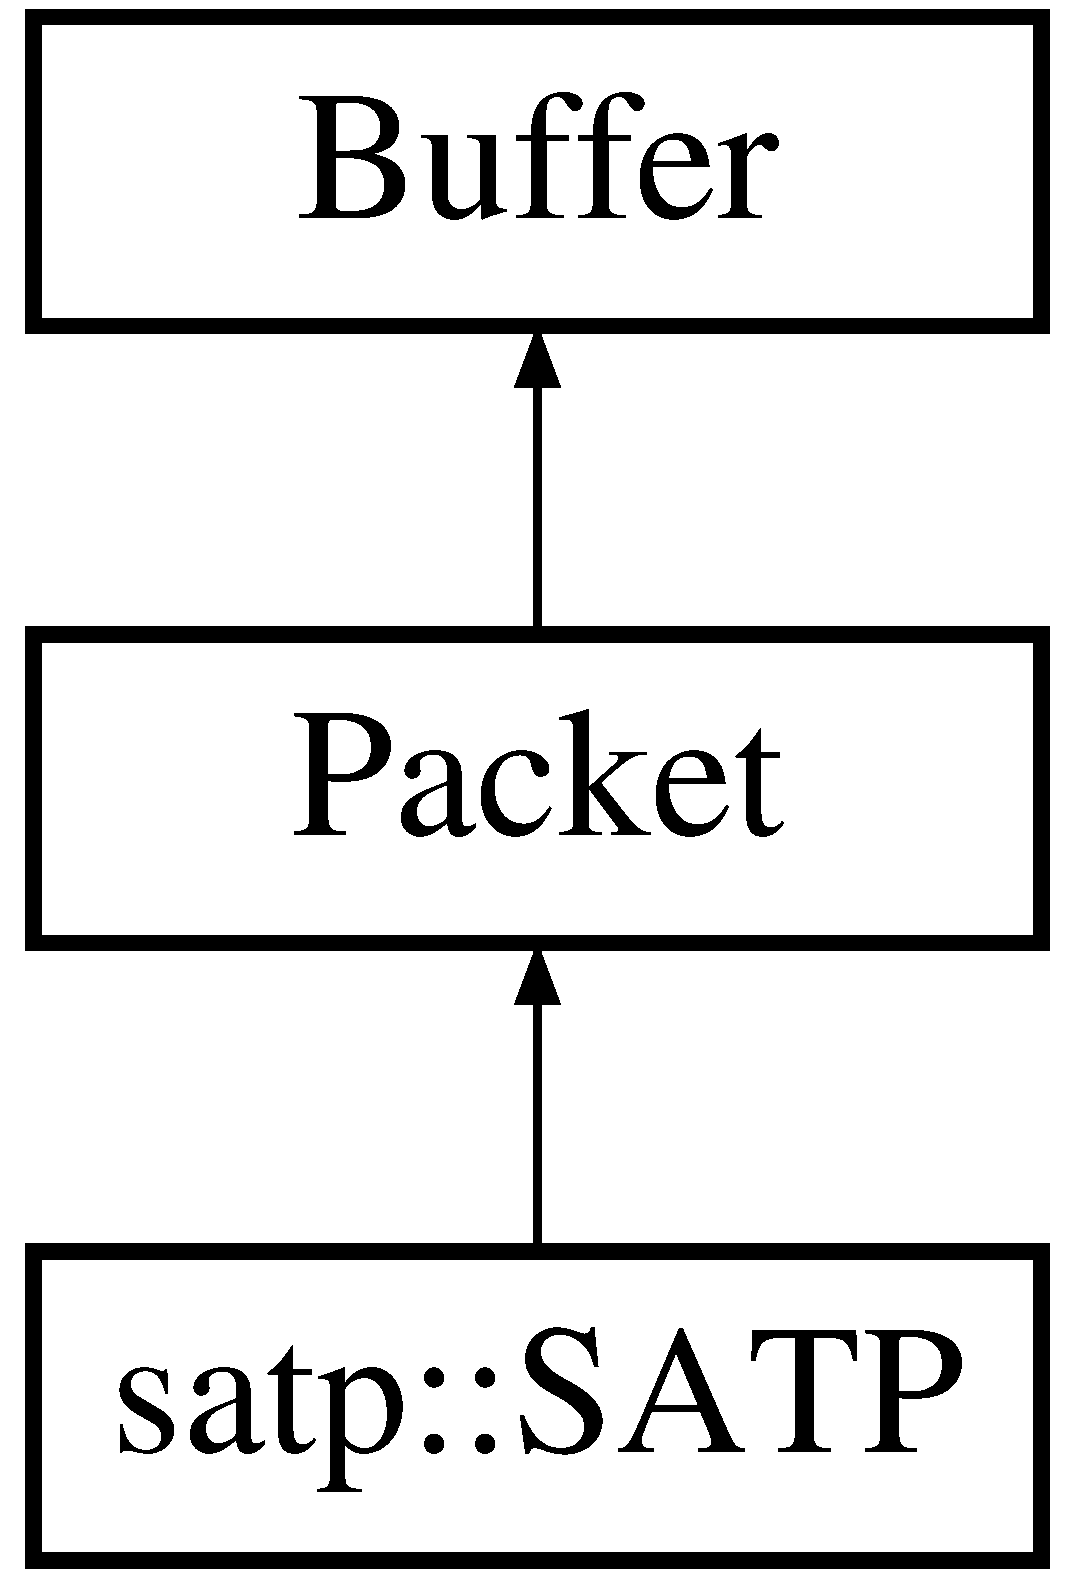
\includegraphics[height=3cm]{classsatp_1_1SATP}
\end{center}
\end{figure}
\subsection*{Static Public Attributes}
\begin{CompactItemize}
\item 
string {\bf name} = \char`\"{}SATP\char`\"{}
\item 
list {\bf fields\_\-desc}
\end{CompactItemize}


\subsection{Member Data Documentation}
\index{satp::SATP@{satp::SATP}!name@{name}}
\index{name@{name}!satp::SATP@{satp::SATP}}
\subsubsection{\setlength{\rightskip}{0pt plus 5cm}string {\bf satp::SATP::name} = \char`\"{}SATP\char`\"{}\hspace{0.3cm}{\tt  [static]}}\label{classsatp_1_1SATP_e9e415324a6a9fbe14971c1ffd334139}


\index{satp::SATP@{satp::SATP}!fields_desc@{fields\_\-desc}}
\index{fields_desc@{fields\_\-desc}!satp::SATP@{satp::SATP}}
\subsubsection{\setlength{\rightskip}{0pt plus 5cm}list {\bf satp::SATP::fields\_\-desc}\hspace{0.3cm}{\tt  [static]}}\label{classsatp_1_1SATP_e51015e8537b5ec7aa53ba87bf638c15}


\textbf{Initial value:}

\begin{Code}\begin{verbatim}[
            IntField("seq", None),
            ShortField("id", None)
            ]
\end{verbatim}\end{Code}


The documentation for this class was generated from the following file:\begin{CompactItemize}
\item 
{\bf satp.py}\end{CompactItemize}
